Our work focuses on providing the benefits of having a standard and matured language as \ac{sql} to serve as querying interface for a \ac{vlsd}. First we needed a query engine, which is the primary interface to the storage engine and uses \ac{sql} as query language. Generally a query engine is composed by two main stages, the compilation and the execution of the query, being that the first is the one in which most optimizations and the choosing of which algorithms to use according to the estimate cost of each operation take place. The second phase is responsible for the actual implementation of algorithms that manipulate the data of the database, such as the scanning of relations which is essential to access the tuples of a relation, and it can be of three types\footnote{These definitions came from conversation with Francisco Cruz}:

\begin{description}
	\item[Table-scan] Reads each block holding the tuples of a relation
	\item[Index-scan] If there is an index on the table it may be used to retrieve the tuples of a relation 
	\item[Sort-scan] Takes as a parameter the sorting attributes, and produces the result in the desired order
\end{description}

The implementation of the algorithms is where most of our work lies, providing a separating layer from the query engine to the underlying storage engine.

As a query engine we chose Apache DerbyDB which is a full fledged open-source Java \ac{rdbms}, that has a very small footprint\footnote{about 2.6MB of disk-space for the base engine and embedded \ac{jdbc} driver~\cite{derbySite}}.

To store the data we chose the \ac{vlsd} Apache Cassandra that was detailed in section \ref{sec:cassandra}.

\begin{figure}[!ht]
  \begin{center}
    \leavevmode
    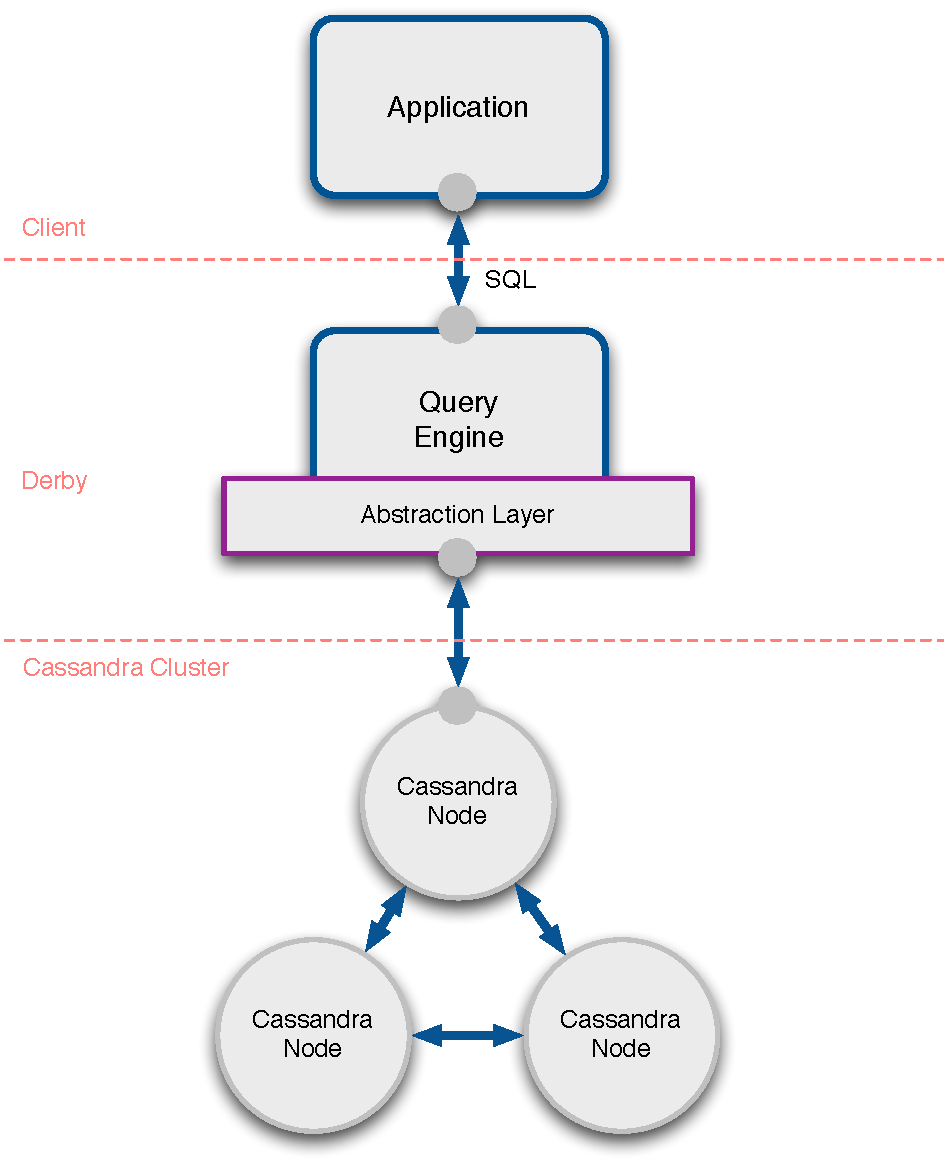
\includegraphics[width=0.9\textwidth]{images/arch}
  \end{center}
  \caption{Derby over Cassandra system architecture}
  \label{fig:derbyCassandra}
\end{figure}

The system architecture is shown in figure \ref{fig:derbyCassandra} and it encompasses an application that has an \ac{sql} interface with the query engine, in this case Derby, which then transfers control to our abstraction layer that will randomly choose a cassandra node from to cluster, connect to it and perform the desired operations. This chapter will focus on the abstraction layer and how it translates the requests into Cassandra's methods.


\section{Abstraction Layer}

The implementation of the abstraction layer involved integrating Derby with Cassandra. On the Derby side this meant changing the way the algorithms are implemented in the storage engine, on Cassandra's side this meant doing two things, defining the way data will be stored and translating Derby operations to its API.  

\subsection{Derby}
\label{sec:patch}

As described above our work prime emphasis is on Derby's storage engine, therefore, before explaining the modifications made there is a need to understand its basic structure.

The Derby engine is composed by multiple packages from which we will focus mainly on the one called \emph{store}, that as the name may suggest is the responsible for the implementation of the storage engine algorithms. Within it lies another package, called \emph{access}, with the specific implementation of said algorithms for each kind of storage\footnote{BTree and Heap are the default ways for interacting with storage in the vanilla Derby}. As would be expected, we wrote similar packages within the access that, when the table name starts with \textbf{TUPLE} (this is our convention), use Cassandra as storage engine. We have named these packages \emph{tuplestore} and \emph{tuplestoreindex} for, respectively, the operations with regular records and with indexes.    

Following Derby's implementation, each type of action has a responsible class, such as the TupleStore for the creation and deletion of tables, the TupleStoreController for insertion, update or deletion of rows and the TupleStoreScanController for fetches that need some sort of scanning. The same applies to index, but the with the suffix Index.

When developing this layer some optimizations were made such as the reutilization of connections, since Derby creates one physical connection to the underlying database for each transaction this can mean a reasonable overhead when a new transaction is created due to the cost of establishing the connection. To circumvent this, a pool of connections is created and if there is one free it is used, otherwise a new connection is opened, which will prevent some of the overhead. 

\subsection{Adopted data model}
\label{sec:data_model}
The way the data is organized in Cassandra is a very important feature of this work and influences the design of the integration with Derby. This was, therefore, something that had to be carefully thought from the ground up. The various design decisions and the reasons supporting them will be thoroughly explored through the rest of this chapter.

This model is not application specific and as such is optimized to the extent it can go without losing its generality. Having this in mind, our design uses one keyspace per relational table, named ``TableXXXX'' with XXXX being the table's conglomerate id\footnote{Derby calls tables and indexes conglomerates, and each of them has a unique id, in our case we use the table id to uniquely identify a keyspace}, with each of these keyspaces having one column family, if it is referring to a table conglomerate it is called \emph{BaseColumns\_CF} and if it refers to an index conglomerate it is called \emph{BaseRowLocation\_CF}.

The rows in each of the previously mentioned column families have a particular structure. In the case of \emph{BaseColumns\_CF}, the row key is the primary key and the row has one column with name ``valueX'', where X is the position of the relational column, for each value inserted. In the case of \emph{nulls}, that are required by \ac{sql} statements, they are simply ignored, as there is no need to create a column for them since Cassandra has no fixed schema.  

The indexes column family deals with two different situations, when it is a unique secondary index and when it is a non-unique secondary index. In both cases, all columns except one have the name ``keyX'', which follows the same logic as ``valueX'', also the row key is the indexed value or values\footnote{rows with secondary indexes can be indexed on multiple values}. In one hand, when the index is unique, the different column has the name ``location'' with the location of the actual record as a value. On the other hand, when it is a non-unique secondary index, the same column has the location of the record as name and no value (Fig. \ref{fig:mymodel}).

\begin{figure}[htb]
  \begin{center}
    \leavevmode
    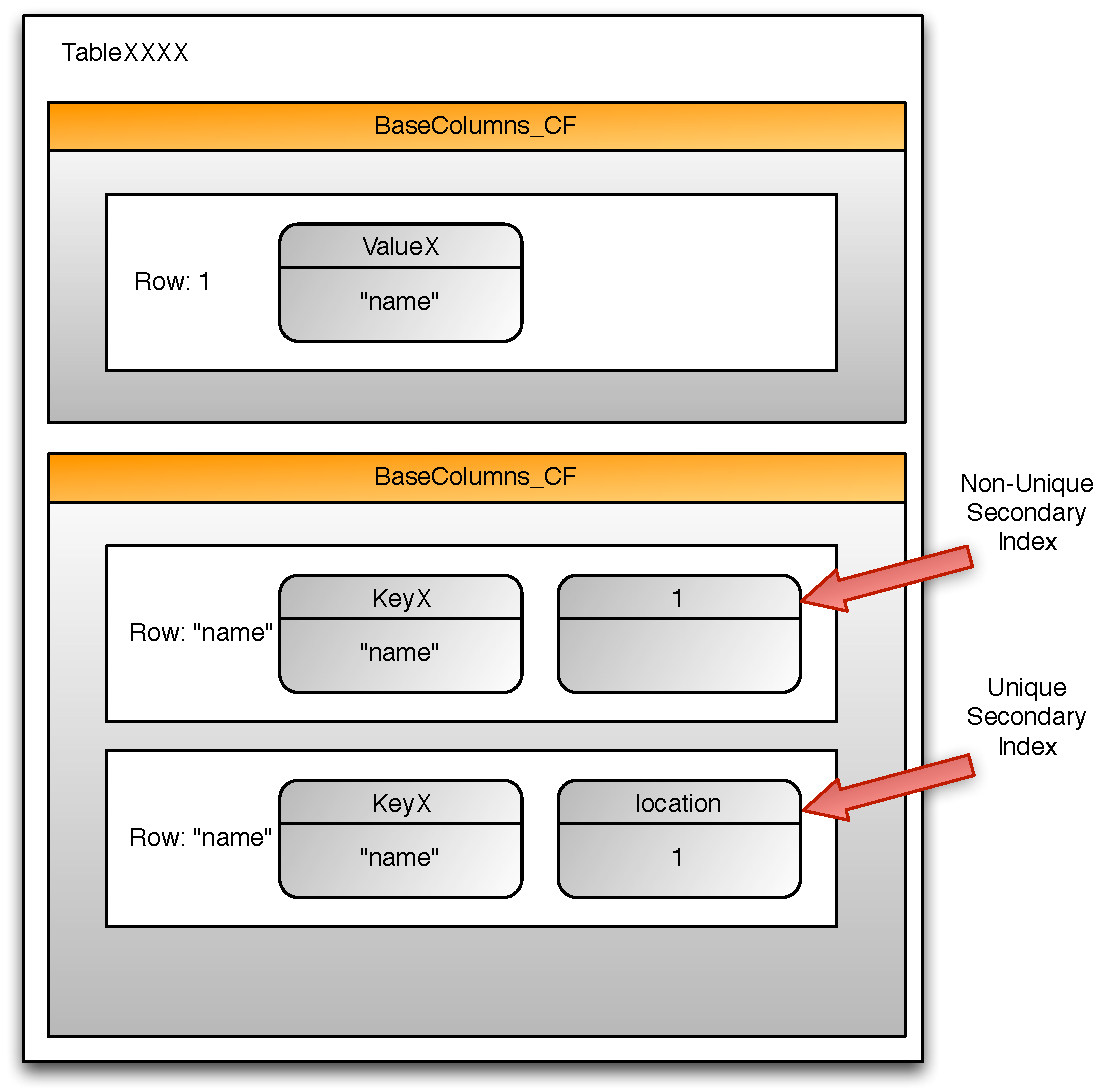
\includegraphics[width=0.7\textwidth]{images/mymodel}
  \end{center}
  \caption{Cassandra design to integrate with Derby}
  \label{fig:mymodel}
\end{figure}

\subsection{Records}
\label{sec:records}
A record, row or tuple all have the same meaning, they represent a container of values, typically in fixed number and indexed by names. In this specific context, they represent a structured data item that is stored in a database table. They are the assets we intend to maintain durable and consistent.

This means that when an insert or update action is performed one or more of these records must be created or updated, alongside with their corresponding indexes, as explained in section \ref{sec:derby_index}.

The various Derby operations that interact with the underlying data store had to be rewritten to be compliant with Cassandra. These operations encompass the creation and deletion of keyspaces, the insertion, replacement, fetching and deletion of rows, as well as the scans or range queries.

\subsubsection{Keyspace operations}
Since version 0.7 of Cassandra it is possible to alter keyspaces definitions on runtime, which allows us to create and delete them\footnote{keyspaces correspond to the relational tables and indexes, in our implementation}.

Therefore, when an \ac{sql} create table statement is issued, a keyspace is created, with the name defined according to the model and the replication factor and strategy coming from a configuration file. At the moment of creation of a keyspace, the respective column family is also created, taking into account if it is an index or not. The deletion is achieved through a call to the provided \emph{system\_drop\_keyspace} method.

While testing the system, we found some problems with these \emph{system} methods that allow the alteration of keyspaces. The main problem is that when a new keyspace is created, the method does not wait for the schema to agree. While this provides better performance since it does not block, it also means that if you try to do a query or an insert on that keyspace before the agreement of the schema, you will get an error that the system cannot come back from. We had to create our own method to wait for the schema agreement to avoid this errors.      

\subsubsection{Row operations}
The operations performed to a row are insert, replace, fetch and delete and as in the keyspaces they differ from indexes to normal records.

The insertion of a row consists on creating a column for each value, following the data model, and doing a batch update. For this operation the differences between indexes and normal records are not many, and are defined in section \ref{sec:data_model}. 

The replacement of a row only makes sense on normal records, since the indexes are managed internally. There are two main types of row replacements, when the primary key is going to change and when it is not. If the primary key changes and has a secondary or unique index, it is deleted and the new row is inserted (which will update the indexes), if it is not the new columns are added to Mutations and applied in a batch. Since this does not alter the primary it key, there is no need to update the indexes. In the first case, if the new row is not complete, the missing values must be fetched in order to complete it.

When fetching a row Derby gets the row for that index from which it extracts the location of the actual record and then does a second fetch, this time to the location pointed by the index. In figure \ref{fig:derbyindexes}, for example, Derby would fetch the row for index \emph{x} and get the location \emph{j}, from which it would get the \emph{info} from row \emph{j} in the records table.

This is fine for unique and secondary indexes, but as explained in the previous section, in the case of primary indexes there is no need for the creation of a specific row for the index, thus making this two fetches mechanism redundant. Since this redundancy meant an unnecessary access to the database, which could incur in a large overhead, this matter had to be addressed. 

The way this was solved was by storing in memory the whole row fetched in first place (through the index) and passing it on alongside with the actual record location. This allows for the tuple controller that is doing the fetch to use the information in memory, when it is available.

For the other types of indexes the location of the actual record must be fetched as well. In the case of unique indexes the column with name ``location'' is fetched and in the case of non-unique secondary indexes the remaining column has the location as its name. This location is added to the previously constructed row that is then validated and returned.

\begin{figure}[!h]
  \centering    
  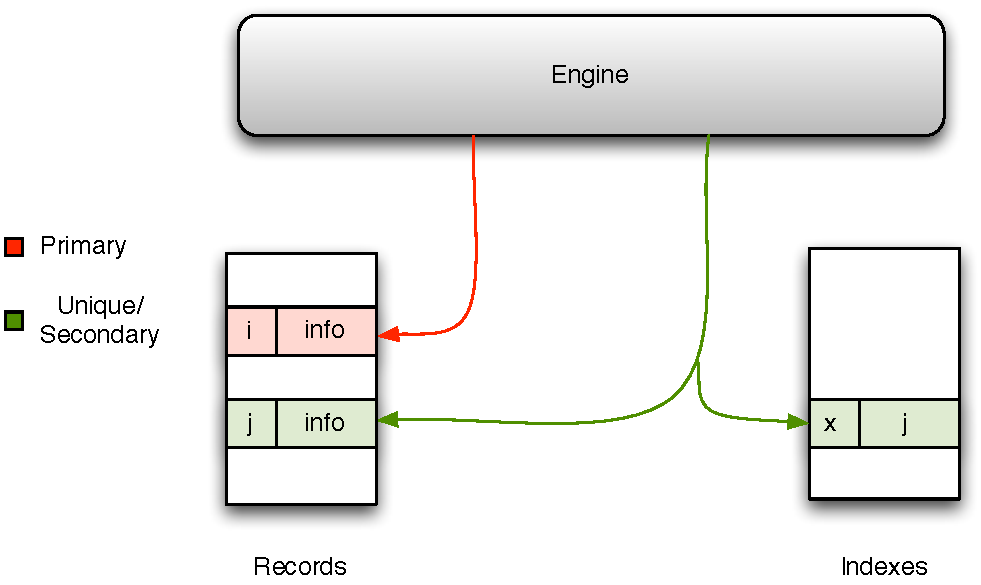
\includegraphics[width=0.9\textwidth]{images/derbyindexes}
  \caption{Derby Indexes}
  \label{fig:derbyindexes}
\end{figure}

In those cases where this optimization cannot be applied, what happens is that the necessary values (it is not mandatory to query for the entire row) are fetched and a Derby row is created and passed on.  

Rows are deleted with Cassandra's method \emph{remove}, which marks them as deleted for a certain time\footnote{this amount of time is called \emph{GCGraceSeconds} and is defined in cassandra's configuration file}. The reason a row is not deleted immediately is because of the fact that the \emph{remove} is actually performing a distributed delete, which means that some of the replicas may not receive the delete operation. In that case, if the data was to be deleted at once, when one of those replicas became available again it would treat the replicas that received the delete as having missed a write update, and repair them. That is why deleted data is replaced with a special Cassandra value called tombstone, that can later be propagated to the replicas that missed the initial remove request.

The reason for this tombstones to be available for a pre defined amount of time is that in a distributed system without a coordinator, it is impossible to know the moment when all the replicas are aware of the delete and it is safe to remove the tombstone. By default Cassandra waits ten days before removing them.


\subsection{Indexing}
\label{sec:derby_index}
Indexing is a way of sorting records on multiple fields. Creating an index on a field in a table creates another data structure with the field value, and a pointer to the primary record. 

The downside to indexing is that these indexes require additional space on the disk and processing time when inserting, updating or removing new data.

\subsubsection{Derby Indexes}
Along with the actual record handling classes, there are the ones responsible for the indexes, which can be of one of three types:

\begin{description}
	\item[Primary] Refers to primary keys. There can only be one per table and it must unambiguously match one, and only one, record.
	\item[Secondary] Secondary or Ordinary indexes are used to accelerate the process of finding a requested row's location by a given value in those cases where this value is not the primary key. 
	\item[Unique] Resemble ordinary (secondary) indexes, except they prevent duplicates from being added.	
\end{description} 

The creation of an index in our version of Derby depends on its type. 

When it is a primary index, Derby is informed about it (through a flag), but no actual index record is created in Cassandra, since in Cassandra it is mandatory for each row to have a key that in this case will be the primary key, and the rows are automatically indexed by that key (Fig. \ref{fig:derbyindexes}).

On the rest of the cases, an index is created according to the model defined in section \ref{sec:data_model}.

When fetching information that is indexed, Derby (as most \acp{rdbms}) first estimates the cost of fetching using the index or not, based on the number and size of the rows, and acts accordingly.

\subsubsection{Indexing in Cassandra}
Secondary indexes where introduced to Cassandra in version 0.7, they allow querying by value and can be built in the background automatically without blocking reads or writes. 

We have not used this, however, because there are still several limitations such as not being recommended for attributes with high cardinality, i.e. attributes that have a lot of unique values, and with these indexes only equality queries can be done, not range queries~\cite{secindexlimitations}.

In the cases where these limitations cannot be tolerated (such as ours) the documentation recommends using a separate column family and implement our own secondary index~\cite{secindex}. 

\subsection{Scans}
\label{sec:derby_scans}

A scan or range query, is the action triggered when the submitted query has inequality operators\footnote{$<$, $>$, $<=$ and $>=$} or uses the \emph{BETWEEN} or \emph{LIKE} operators.

In Derby, the range to which the query applies is passed on to the scan controller through a start and a stop key and a flag that defines if the range is inclusive or exclusive in either end. With this parameters, the controller fetches the needed rows to memory, validates each one and returns those which are valid.

\begin{figure}[!h]
  \centering    
  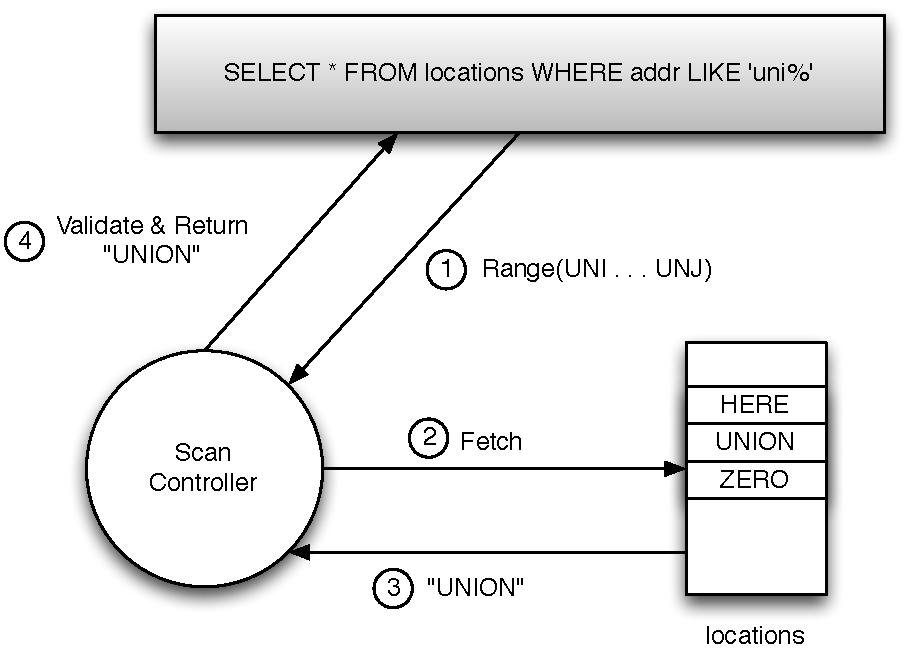
\includegraphics[width=0.7\textwidth]{images/likescan}
  \caption{Querying with \emph{LIKE}}
  \label{fig:likescan}
\end{figure}

As can be perceived from figure \ref{fig:likescan}, there are two assumptions that must be met in order for a \emph{LIKE} query to function properly.

\begin{enumerate}
	\item The keys must be ordered by their byte value, so that strings as well as integers and any other type of data are logically ordered\footnote{If they were ordered by their UTF-8 value, for example, the number 10 would be between 1 and 2, which means that a query for all records which have a value between 8 and 10, would return 2 records (8 and 9) instead of the expected 3 (8, 9 and 10)}.
	\item The encoding of the data types must be coherent throughout the application 
\end{enumerate}

The first assumption was met through the Ordered Partitioner that comes bundled with Cassandra, as was explained in section \ref{sec:partitioners}. The second one meant having classes to encode each type of data that Derby accepts (Integer, Float, String, DateTime, etc\ldots), as well as altering the way padding is applied to the strings that are received through a \emph{LIKE} query so that it becomes compliant with the way Cassandra stores its data. This has to be done because Cassandra does not allow for range queries on string prefixes. Take the example in figure \ref{fig:likescan}, for instance, the values in the range in step one have to be padded so that they have at least the same length as the value we are looking for, in this case \emph{UNION}. 

Both with normal records and indexes the primary method is \emph{fetchNext}, which returns the next row in the range. In the case of records this consists in getting the next row from the iterator and encoding the values to create a Derby row. 

\subsubsection{Scanning with indexes}

Performing a scan that involves fetching a row through an index is a bit more complex since the indexes can be of three types, which means doing things a little different for each of the types. 

When performing a scan that involves fetching a row through an index, Derby fetches row by row according to the mechanism in section \ref{sec:records}.

When performing scans in Cassandra there is one other detail to take in account, that is the fact that a column (or row) is only deleted after a certain amount of time, which means that some tombstones\footnote{special markers for columns that have been deleted} may be returned, these are known as range ghosts. Cassandra had a range query method that eliminated tombstones from the result set, but has been deprecated due to performance issues, therefore when iterating over the rows it is necessary to be aware that a row coming from a range query can have no columns at all if it has been deleted and is now a tombstone or just some of the columns have actual valid values.  



